\section{Introduction}
\label{sec:intro}

%Opinions about a certain named entity,
%such as a famous person, a world-wide organization, or a place,
%may differ from culture to culture.
%For example, Kashmir is a large mountainous region on the China-India border.
%Due to decades of border disputes between China and India
%about that region, to the Chinese people, this region is
%synonymous to military conflicts and political struggles.
%On the contrary, that same region is considered as a picturesque travel
%destination by the westerners due to its perfect location in the Himalayas,
%since the border dispute between China and India is hardly their concern.
%This type of cultural differences are evident from the most popular
%images about Kashmir on the English and Chinese search engines
%(\figref{fig:kashmir}).

%Another type of cultural differences exist when an entity is interesting
%to one culture but largely ignored by another culture. \figref{fig:bjp}
%shows such an example where Indian People's Party
%(a.k.a. Bharatiya Janata Party or BJP), currently the largest political
%party in India, shows up frequently on Chinese web with vivid rally images,
%because India is a major world power that sits next to China. On the
%other hand, the most popular English web images about BJP are
%merely party logos, suggesting very little public interest about this
%entity from the English world.

%\begin{figure}[th]
%	\centering
%    \begin{subfigure}{0.32\columnwidth}
%        \centering
%        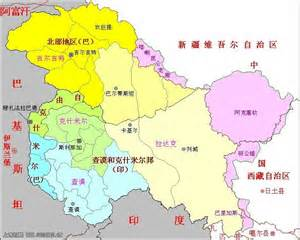
\includegraphics[width=\columnwidth]{figures/keshimier1.jpg}
%    \end{subfigure}
%    \begin{subfigure}{0.32\columnwidth}
%        \centering
%        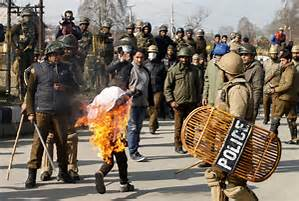
\includegraphics[width=\columnwidth]{figures/keshimier2.jpg}
%    \end{subfigure}
%	\begin{subfigure}{0.32\columnwidth}
%        \centering
%        
\includegraphics[width=\columnwidth]{figures/keshimier3.jpg}
%    \end{subfigure}
%	\centering
%    \begin{subfigure}{0.32\columnwidth}
%        \centering
%        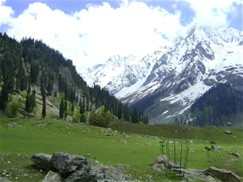
\includegraphics[width=\columnwidth]{figures/kashmir1.jpg}
%    \end{subfigure}
%    \begin{subfigure}{0.32\columnwidth}
%        \centering
%        
\includegraphics[width=\columnwidth]{figures/kashmir2.jpg}
%    \end{subfigure}
%	\begin{subfigure}{0.32\columnwidth}
%        \centering
%        
\includegraphics[width=\columnwidth]{figures/kashmir3.jpg}
%    \end{subfigure}
%\caption{Popular Images about Kashmir on Chinese web (top) and
%English web (bottom)}
%\label{fig:kashmir}
%\end{figure}
%
%
%\begin{figure}[!ht]
%	\centering
%    \begin{subfigure}{0.32\columnwidth}
%        \centering
%        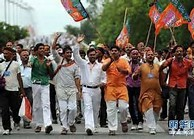
\includegraphics[width=\columnwidth]{figures/yindu1.jpg}
%    \end{subfigure}
%    \begin{subfigure}{0.32\columnwidth}
%        \centering
%        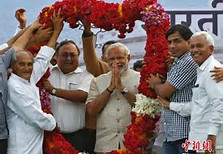
\includegraphics[width=\columnwidth]{figures/yindu2.jpg}
%    \end{subfigure}
%	\begin{subfigure}{0.32\columnwidth}
%        \centering
%        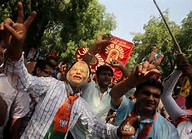
\includegraphics[width=\columnwidth]{figures/yindu3.jpg}
%    \end{subfigure}
%	\centering
%    \begin{subfigure}{0.32\columnwidth}
%        \centering
%        
\includegraphics[width=\columnwidth]{figures/bjp1.jpg}
%    \end{subfigure}
%    \begin{subfigure}{0.32\columnwidth}
%        \centering
%        
\includegraphics[width=\columnwidth]{figures/bjp2.jpg}
%    \end{subfigure}
%	\begin{subfigure}{0.32\columnwidth}
%        \centering
%        
\includegraphics[width=\columnwidth]{figures/bjp3.jpg}
%    \end{subfigure}
%	\caption{Popular Images about BJP on Chinese web (top) and
%English web (bottom)}
%	\label{fig:bjp}
%\end{figure}

%Our goal in this paper is to identify an entity with significantly different
%cultural understanding, which can contribute to applications such
%as instant messenger or machine translator,
%to avoid culturally sensitive mentions or translations.
%Apart from these applications, a list of such entities with
%cultural differences in its own right is a valuable resource for
%multicultural studies.
%However, understanding subtle cultural differences requires not
%only perfect understanding of the two languages, but also devouring
%large volumes of bilingual texts to sufficiently observe how
%they are mentioned in each culture and how they differ.
%
%We propose to transform this problem into a computational task,
%by proposing a quantitative evaluation metric measuring
%the cultural similarity between two cultures of a given named entity.
%To calculate such scores, we proposed two algorithms to compute
%the cultural similarity scores based on the quantitative representation
%for the semantic meaning of all words in mono-lingual corpus.
%First solution leverages
%word-embedding techniques such as word2vec, to mine the notion of similarity from English and Chinese corpus respectively.
%We then connect the two results using linear transformation so that we can directly compute the cosine similarity between the English name and the Chinese name of a certain named entity.
%
%%Bill: I think two paragraphs are more comfortable to read
%Another way is to construct a higher-dimensional vector space.
%Every dimension of this space is representing a pair of words,
%which are an English word and its corresponding Chinese translation.
%We call this space ``translation space''.
%The values in the English name vector of a certain entity are
%the cosine similarities between
%this entity's English name and each of other English words.
%We similarly compute the Chinese name vector.
%Because an English word may has many different Chinese translations, we duplicate the cosine similarities into several dimensions in translation space. After constructing this new comprehensive vector space, we can simply calculate cosine similarity between the English and Chinese vector of a certain entity.
%The last method is also based on the comprehensive semantic space we just constructed, but we focus instead on the top K highest dimensions to calculate the Jaccard similarity between the two name of a certain entity.

%We proposed three algorithms calculating the scores, which are all based on word-embedding technique.
%Contribution

% in opinions and concerns towards named entities (persons, places and organizations.) 
%Apart from that, social
Computing similarities between terms is one of the most fundamental
computational tasks in natural language understanding. Much work has been done
in this area, most notably using the distributional properties drawn from large monolingual textual
corpora to train vectorial representations of words or other 
linguistic units~\cite{Bengio2000ANP,pennington2014glove,Le2014DistributedRO}. 
Recently there is growing interest in cross-lingual and cross-cultural similarity computation \cite{luong2015bilingual,Garimella2016IdentifyingCD,camacho2017semeval}.
%ruder2017survey
In this paper, we consider interesting questions like these:
%Consider the following questions. 
\begin{enumerate}
\item {\em Is there any cross-cultural difference between Nagoya 
(a city in Japan) for native English speakers and 名古屋 (Nagoya in Chinese) for Chinese people?}
\item {\em What are the English terms that can explain the meaning of ``浮云'' (a Chinese Internet slang term)?}
\end{enumerate}
Such questions are important in cross-cultural social studies 
and machine translation systems for producing culturally sensitive results.  
We can generalize these two questions into two
cross-cultural and cross-lingual tasks.  

The first task is mining cross-cultural differences in
the perception of named entities (e.g., persons, places and organizations). 
Opinions about named entities can be very different from culture to culture. 
%especially on social media where people feel free to share their views. 
Back in 2012, in the case of ``Nagoya'', while most native English speakers considered 
the city to be a nice travel destination, 
Chinese people overwhelmingly greeted the city with anger and 
condemnation because the city mayor denied the
truthfulness of the Nanjing Massacre in 1937. 
Enabling machines to understand
such cross-cultural differences toward named entities can be useful in various
cross-lingual language processing tasks and human-computer interactions.
%This example suggests that a literal translation at this time may be culturally insensitive. 
%\BL{but we didn't focus on translation of this kind. I think we just need to prove the difference exists.}
%Therefore, automatically recognizing such cross-cultural differences of named entity from social media is important in effective cross-cultural studies and communications. Additionally, identifying named entities with significantly cross-cultural understanding can help intelligent systems such as Machine Translation and Multilingual Knowledge Graph incorporate cross-cultural understanding. Simply put: MCDNE task is to quantify the semantic similarity of a given named entity in different cultures with a score.

The second task is to explain slang terms across languages. 
Social media is a rich soil to produce novel slang 
terms in all cultures. 
For example, ``浮云'' literally means ``floating clouds'', 
but now it almost always means ``nothingness'' on the Internet; 
``天朝'' literally means ``Heavenly Kingdom'', 
now becomes a common nickname for the Chinese government.
Experiments show that state-of-the-art machine translators 
often translate such slang terms to their literal meanings, 
even under a clear context where slang meanings are much more appropriate.
%We wish to automatically derive a bilingual lexicon that includes normal
%words in one language to explain such dynamic slangs in another language.
Simply put, given a slang term in one language, this task is to find
some terms in another language which can help explain its meaning. 

Both of the two tasks share a core problem, which is \textit{how to compute 
cross-cultural differences (or similarities) between two terms from 
different languages}.
\footnote{A term here refers to either an ordinary word, an entity name or a slang term. }
%\KZ{without losing socio-linguistic characteristics}


Existing bilingual word representation models require bilingual supervisions: 
aligned parallel corpora with alignments, bilingual lexicons or 
comparable documents~\cite{upadhyay2016cross}.
%Existing approaches~\cite{Sarath2014An,kovcisky2014learning} are primarily 
%These resources are very costly to obtain and the approaches often don't scale.
However, aligned parallel corpora from social media are usually expensive to
obtain and do not scale. Plus, most models do not purposely preserve 
features reflecting social and cultural contexts in different cultures.

In this paper, we propose a novel approach to project 
two heterogeneous monolingual word vector spaces into 
one bilingual word vector space, known as 
social vector space (\textit{\socvec}), 
by constructing a bilingual social lexicon (BSL), which
contains a set of bilingual mappings of selected words
that reflect opinion, sentiment, cognition and many other psychological 
processes. 
These words, we believe, are central to capturing cultural
differences~\cite{Garimella2016IdentifyingCD}.
%using only a bilingual lexicon (for common words), two monolingual socio-linguistic vocabularies and a comparable corpus\footnote{A comparable corpus is a pair of corpora in two different languages, which come from the same domain.} from microblogs, all of which are easily available.
Each dimension of our \textit{\socvec}~then represents a feature 
derived from mono-lingual semantic similarities between an input term and 
each entry of the BSL. 
Consequently, a term $W$ in language $L_1$ and a term $U$ in 
language $L_2$ can each be respectively projected 
into a bilingual word vector in the \textit{\socvec} while maintaining
their social features. Thus the cross-cultural similarity 
between $W$ and $U$ can be computed directly with the two vectors 
from the \textit{SocVec}. 
%Thanks to the large size of our social word vocabulary and the developing process,(around 3k-5k)  
Note that \textit{ScoVec} is an encoding for words across languages, where each dimension has 
clear meaning. Such encoding methods have been shown to be beneficial in 
cross-lingual transformation and multilingual tasks~\cite{DBLP:journals/tacl/Berend17,DBLP:journals/corr/SmithTHH17}.
%To reflect cross-cultural differences of  terms in such a projection,
%we make use of a set of words 
%This approach is backed by the following observations: i) the opinions and sentiment toward a concept or an entity
%can be captured by opinion-related context; 
%ii) such social contexts can be mined from
%online social media such as Twitter and Weibo;
% iii) public opinion changes over time, so one can only
%talk about cross-cultural differences with respect to a 
%particular time frame. 
%\BL{still feel strange here, we may remove point 3 to 3.1 data preparation }
%\BL{ Observation 3 is true but it seems not related to using  
%opinion-related words} 

%In the constructed SocVec space, we can directly compute distances or similarities 
%between any two words from different languages, which solves the core problem stated 
%above and thus the two tasks will be readily induced. 
%\SH{However, understanding cross-cultural differences often requires a cross-lingual comparison of
%distributional hypothesis. Meanwhile, it is challenging and no one has done...}
%For it is a ubiquitous technique of central importance in Natural Language Processing (NLP), 
%vector-space word embeddings are essential to data-driven cultural study and 
%sociolinguistic research. However, when it comes to \emph{cross-lingual} research, 
%it is challenging to implement a model to induce cross-lingual word embeddings that 
%can capture the cultural information and sociolinguistic knowledge of high quality without 
%expensive supervision cost like parallel corpus annotated with word alignments.  
%
%
%The goal of this paper is to build effective sociolinguistic models of cross-lingual word vectors (\textbf{SocVec}) with cheap cost and utilize them to attack two novel cross-lingual sociolinguistic tasks as follows:



%As a popular language communication mode, more and more Internet slang keep emerging from social media with the boom of microblogs and thus arouse significant concern in sociolinguistics, web data mining, natural language processing, etc. 
%Taking Weibo as an example, many new Chinese words and emerging meanings are created over time: 
% 
% ``ZF'' (phonetic abbreviation, replacement for ``government'' used by netizens to avoid censors), etc. 
%Many Twitter users use the word ``adorbz'' to express the meaning of extreme cuteness and adorableness, while in Weibo, the Chinese word ``萌'', which literally means ``sprout'', is now widely used like the English term ``adorbz'' and ``cute''. 
%Netizens sharing same language or culture have their own Internet slangs, 
%while it is difficult to explain their meaning and find their counterparts in other languages. 
%\BL{these two examples could be brought earlier. }

%To fill this slot, BLEIS task aims to find the cross-lingual counterparts of a given Internet slang, which are expected to be either formal words or Internet slang in another language. 

%Rule-based systems are impractical for both tasks, since they require not only 
%perfect understanding of both formal and informal language use, but also devouring large 
%volumes of bilingual texts. At the same time, lacking large-scale annotated text data, 
%we cannot consider them to be supervised machine learning tasks. 

%\SH{new para? we need to define "sociolinguistic knowledge" In contrast, we aim at a direct and uncomplicated approach, for which we identify the following research question:}
%While seeking a direct and uncomplicated approach, we attempt to solve the core problem shared by both of the tasks: 
%\textit{How can we compute semantic similarity cross-lingually with 
%sociolinguistic information?} 
%For MCDNE task, we can directly compute the distance between Nagoya and ``名古屋'' (Chinese name of Nagoya) in SocVec space and use the distance to quantify the differences of Nogoya between Chinese and Western culture; As for BLEIS, we are able to find the most similar English words to ``浮云'' in SocVec space as its counterparts. 
 
%We first collect a English lexicon consisting of $N$ words relevant to psychological processes and opinions. In terms of another language, we obtain a translation version of this lexicon with the help of a bilingual lexicon.  Each dimension of this Social Space is a sociolinguistic feature is basically the semantic similarity between the source vector and the corresponding word vector to each dimension.  For example, 

%Netizens use Internet slang so frequently for several reasons: 1) Internet slang communicates nuances of meaning or emotion better than formal words. \BL{example of FuYun} . 2) Another important purpose, especially of Chinese netizens, is to avoid censorship from authorityz. \BL{example of ZF and TianChao} 

 
%Related Work Section

%Previous work show that monolingual word vectors can be improved by incorporating cross-lingual distributional information. \cite{Klementiev:2012uk,Mikolov:2013tp} \BL{cite more later} There are plenty work focusing on using cross-lingual information to improve the performance of monolingual tasks such as word semantic similarity. \BL{cite more later} However, there is little work aiming to quantifying cross-cultural similarities and differences of named entity through such cross-lingual word vectors directly.
%
%On the other hand, although there are indeed many researchers utilizing cross-lingual word vectors to attack the Bilingual Lexicon Extraction problem (\BL{cite more later}), all of them are dealing with formal source words and formal target semantics of source words. An automated approach to mining the most related English words of Chinese Internet slang . through calculating similarity within cross-lingual  is missing from literature 
In summary, this paper makes the following contributions:
\begin{enumerate}
\item We propose a direct and uncomplicated bilingual word 
representation model as a building block
for cross-cultural social studies with low-cost bilingual resources. 
\item We propose two novel and important tasks in computational social 
science and evaluate our model on both of them. Experimental results
show that our model outperforms strong baseline methods 
by significant margins. 
%with human perception for MCDNE, with an
%average precision of [xxx] and Spearman correlation of [xxx],
\item We open-source a prototype tool for building \textit{\socvec~} and 
release two valuable datasets on the above tasks as well as 
a bilingual socio-linguistic lexicon, which will benefit future research 
in this area. 
\end{enumerate}
